\capitulo{5}{Aspectos relevantes del desarrollo del proyecto}

En este apartado se recogen los aspectos más importantes. Explicando las decisiones tomadas del proyecto, y las consecuencias que suponen, comentando los errores y como se solucionaron.

\section{Inicio}

Una vez se me explicó la idea que se buscaba con este proyecto, me gustó la idea de poder hacer una aplicación que pudiera servir al sistema sanitario publico.

En este inicio, empecé a imaginarme como podría ser la aplicación haciendo bocetos mentales de sus distintas pantallas, como era muy efímero, se hizo una búsqueda de aplicaciones similares, para comprobar alguna interfaz a añadir, donde se encontró la aplicación RetinCam. Con una idea más formada, se hicieron los bocetos iniciales de la aplicación.
\section{Formación}

Para el proyecto no se necesito una formación especifica, puesto que para la aplicación de Android Studio se usó el lenguaje Java, visto durante la carrera, además también se hizo una aplicación de Android Studio en la asignatura ``Interacción hombre-maquina'' y para la creación de la red neuronal se usó el lenguaje Python, que también se ha visto durante la carrera. 

A su vez, ha sido necesario el uso de tutoriales, y de guías de Android Studio y de keras para implementar correctamente el código.

\subsection{Cámara en Android Studio}

Una de las implementaciones en las que se tuvo que formar fue hacer uso de la cámara en una aplicación, guardando posteriormente la imagen obtenida.

Para ello, primero era inicializar la cámara, que se obtuvo una referencia de la propia Android \href{https://developer.android.com/training/camera/camera-intents}{Hacer foto con la cámara} \cite{android-camera-intents}.

Al implementar inicializar cámara surgió un problema con los permisos de la aplicación, y no se abría la cámara, por lo que se buscó como implementar que se pidieran los permisos de la cámara al usuario, que se obtuvo una referencia de la propia Android \href{https://developer.android.com/training/permissions/requesting?hl=es-419}{Obtener permisos} \cite{android-permissions-requesting}.

Una vez abierta la cámara, se tenia que guardar el resultado, puesto que se hacia la foto, pero no se mostraba al usuario, ni se guardaba de forma interna. Llegando otra vez a la pagina de Android, donde en un ejemplo se podía ver como implementarlo.
\href{https://developer.android.com/training/basics/intents/result?hl=es-419}{Guardar resultado de la actividad} \cite{android-intents-result}. 

Con la imagen obtenida de forma local, solo había que mostrarla al usuario.

\subsection{Galería en Android Studio}

Al igual que en la cámara, no se tenían los conocimientos para implementar este requisito.

Por ello, se utilizó el mismo enlace que en la cámara para obtener los resultados.\href{https://developer.android.com/training/basics/intents/result?hl=es-419}{Guardar resultado de la actividad}\cite{android-intents-result}. 

Para llamar a esta actividad, se usó la respuesta de un foro de \href{https://stackoverflow.com/questions/38352148/get-image-from-the-gallery-and-show-in-imageview}{stackoverflow} \cite{stackoverflow-gallery-imageview}, que permitió llamar de forma correcta a esta actividad.

Como en el caso de la cámara, se pensó que también sería necesario el uso del permiso para leer almacenamiento externo. Surgiendo un error de ejecución. Se pensó que era un error de programación hasta que se encontró el siguiente enlace \href{https://developer.android.com/about/versions/11/privacy/storage?hl=es-419}{Version Android 11}\cite{android-storage-privacy}. En este enlace, se comenta como a partir de la API 30, el permiso para leer almacenamiento externo no es necesario.

Una vez implementado este apartado, se uso correctamente la aplicación.

\subsection{TensorFlow en Android Studio}

Para implementar TensorFlow en Android Studio, se uso su versión para móviles TensorFlow Lite.

Como no se conocía como implementar un modelo, se fue a la guía de TensorFlow Lite, donde recomendaban el uso de un Interprete.
Siguiendo el siguiente enlace como guía \href{https://www.tensorflow.org/lite/guide/inference?hl=es-419}{Guía de TensorFlow Lite} \cite{tensorflow-lite-guide}.

\subsection{Modelo en python}

Para crear un modelo keras en python, se usó la guía que viene en TensorFlow para \href{https://www.tensorflow.org/tutorials/images/classification?hl=es-419}{clasificación de imágenes}\cite{tensorflow-classification-tutorial}.

Posteriormente, se escogió el modelo VGG16 por su conocimiento en el preprocesado, como modelo; por lo que se cambiaron las capas por una llamada al modelo VGG16.

Con el modelo ya creado, se calculo la ``accuracy'' entre un conjunto de modelos, escogiendo el máximo valor, en un conjunto de entrenamiento. 

Aunque en asignaturas de la carrera, se había visto el desbalanceo de datos en la vida cotidiana, al inicio se consideró que no era un desbalanceo tan exagerado.

Este pensamiento se descartó puesto que podría dar problemas a la hora de usar la aplicación. Usando la precisión y ``recall'' como medidas.

\subsection{Otras búsquedas}

Además de las búsquedas mencionadas anteriormente, cabe destacar otros errores, tanto de programación, como de incompatibilidad entre otras cosas; que fueron solucionados por la comunidad de stackoverflow y de YouTube.
\section{Metodologías}

Como ya se ha comentado anteriormente, se decidió utilizar una metodología SCRUM, no siguiéndose al completo, puesto que los equipos de desarrollo en esta metodología están compuesto de 3 a 9 personas, a su vez, hay reuniones que no se han podido realizar, entre otras cosas. Pero, con esta metodología se ha buscado que el proyecto tuviese una metodología ágil.

Un fallo cometido con respecto esta metodología ha sido que los martes cambiaba de sprint a las 8 de la mañana, y la revisión para finalizar el sprint, se realizaba los martes por la mañana, haciendo que algunas veces las tareas cambiasen de sprint cuando no debían, y por tanto, la reunión para comenzar el sprint se realizaba con el sprint comenzado.

Las características ágiles de este proyecto son:
\begin{itemize}
    \item Los sprints planeados han tenido una duración de 2 semanas, entregando un incremento al final de cada uno.
    \item Se han realizado reuniones, tanto para finalizar el sprint, como para el inicio del siguiente, teniendo en consideración el fallo comentado anteriormente.
    \item Las tareas que se planeaban para un sprint, se estimaban y priorizaban en un tablero canvas, tanto físicamente como con la herramienta ZenHub. Aunque con el paso de los sprints, se dejo de hacer físicamente.
    \item Para comprobar el progreso del proyecto, se ha utilizado los gráficos burndown, que aunque los ofrece ZenHub, se han realizado a mano, por el fallo comentado.
\end{itemize}

Al principio del proyecto se planeaba utilizar otras metodologías como \textit{Test-Driven-Development} o como \textit{Data-driven testing}, junto con pruebas automáticas, vistas durante el año académico en la asignatura Validación y pruebas, para comprobar como las implementaciones que se iban realizando en el proyecto no se veían afectadas entre ellas y que se implementaban correctamente. 

Pero al implementar las distintas interfaces, se decidió hacer pruebas manuales, las cuales proporcionan una mayor comprensión de la interacción que tiene el usuario con la aplicación, buscando siempre que el usuario entienda el sistema.

\section{Aplicación Android}

Para trabajar en el proyecto, se pensó en utilizar Android Studio o UNITY, la opción seleccionada fue Android Studio, porque ya se tenían nociones previas. 

Con el IDE seleccionado, se realizó el boceto al igual que se tenía realizado a mano, seleccionando como API para trabajar la versión 21, que como informa Android Studio al crear el proyecto, se puede ejecutar en el 99,5\% de dispositivos \ref{fig:API-Android}.

        \begin{figure}[!ht]
                 \centering
                 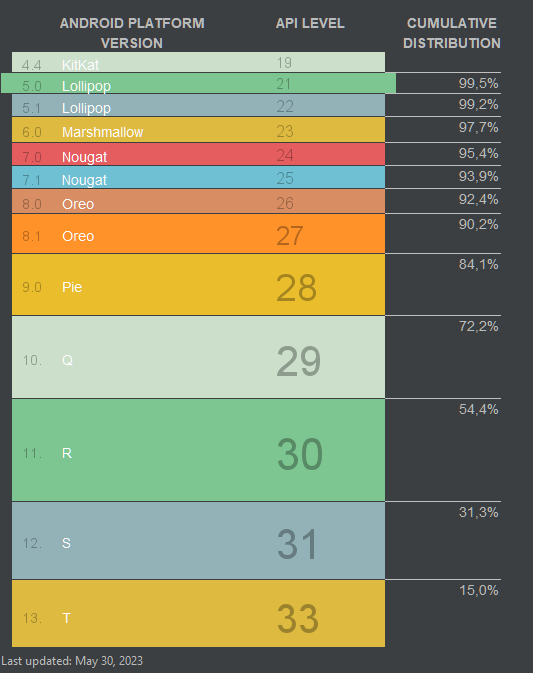
\includegraphics[width=0.45\textwidth]{img/API-android.png}
                  \caption{Porcentaje de dispositivos según la API. Imagen obtenida de Android Studio.}
                 \label{fig:API-Android}
        \end{figure}

Después de terminar el boceto(\href{https://github.com/mfg1014/Retinopatia-diabetica/issues/7}{Issue \#7}), se modifico la interfaz, puesto que en una reunión se propuso añadir y eliminar funcionalidades a la aplicación, en esta reunión se planteó añadir un modo oscuro, añadir la posibilidad de entrar como invitado, añadir una red neuronal que determine la calidad de la imagen, y en caso de ser mala, se repita la imagen, y una opción para cambiar el orden de los ojos, permitiendo que el médico elija su propia preferencia. Estas funcionalidades han sido introducidas en Issues posteriores.

Durante la implementación se encontraron varios bugs, que en algunos casos se encontraban durante la programación de esas partes del código, y en otros casos, se encontraban durante la ejecución de la aplicación de forma normal. De esta forma, en algunos casos se programaron Issues orientadas a la eliminación de estos errores, y en otros casos se hizo sobre la propia Issue que se estaba introduciendo.

Entre los bugs encontrados, cabe destacar los siguientes:
\begin{itemize}
    \item Bug con el modo oscuro entre actividades, al introducir la variable que indicaba que el usuario había activado el modo oscuro, al pasar la variable de una actividad a otra, en algunos lugares estaba mal instanciada y producía errores de ejecución.
    \item Bug con el modo oscuro de texto e imágenes no legibles, cuando se implemento el modo oscuro, algunas vistas de la interfaz no se cambiaron de forma correcta, de forma que el color del fondo no se distinguía de la vista.
    \item Bug con el botón que cambia el orden de los ojos, durante la implementación de esa parte, solo se probó si el botón cambiaba el orden de forma correcta, y así era, pero cada vez que se entraba a esa ventana estaba siempre en la misma posición. 

    \item Bug con LocalDateTime, al principio para introducir en la base de datos la fecha del informe introducido o la fecha de nacimiento de los médicos y los pacientes, se utilizaba la clase LocalDateTime, aunque Android Studio avisaba de que era recomendable no usar esa clase, se utilizó, el problema surgió cuando se probó con un Android con versión API inferior, donde ni inicializaba la aplicación.

    \item Bug con la base de datos, la primera base de datos, era un conjunto de clases java donde con un constructor se inicializaban los usuarios, pacientes, informes,... El problema surgió cuando cada vez que se inicializaba la aplicación se usaba el constructor. Se implementó el patrón singleton y seguía ocurriendo el mismo problema, por ese motivo, se decidió utilizar SQLite para la base de datos.

    \item Bug con la petición de permisos, en la forma que se pedian los permisos, creaba infinitas comprobaciones de los permisos de cámara, haciendo que si no se contestaba durante un tiempo, la aplicación ``crasheará''. Se solucionó eliminando el bucle y pidiendo un sólo permiso a la vez. 
\end{itemize}

\section{Implementación de las redes neuronales}

Al iniciar el proyecto no se tenían conocimientos de TensorFlow, por lo que se tuvo que buscar información sobre como se podría integrar una red neuronal en una aplicación Android. Además las redes neuronales se recomendaban implementar en TensorFlow Lite, por lo que era necesario una conversión del modelo. Por lo que se obtuvo formación de las siguientes páginas:
\begin{itemize}
    \item Cargar un modelo TensorFlow Lite en Android \cite{tensorflow-lite-android-quickstart}
    \item Convertir modelo keras en modelo TensorFlow js \cite{tensorflow-js-import-keras}. Con esta idea, se usó la idea para convertir en formato TensorFlow Lite.
    \item Preprocesamiento modelo VGG16~\cite{tensorflowVGG16}
    \item Preprocesamiento modelo ResNet50V2~\cite{tensorflowResNet50V2}
\end{itemize}

Con la información obtenida de los enlaces anteriores, se hizo un modelo básico que calculaba la operación XOR en la \href{https://github.com/mfg1014/Retinopatia-diabetica/issues/21}{Issue \#21}; para comprobar su correcto funcionamiento.

Posteriormente, se recomendó el uso de la red VGG-16 ya entrenada para comprobar los resultados con imágenes, para ello, se uso la red publicada por Lorenzo Baraldi~\cite{github-vgg16}. Para introducir esta red neuronal se necesita el preprocesamiento de los datos y para su ejecución se necesita saber el numero de salidas de la red; esta red esta destinada a el conjunto de datos ``imagenet''~\cite{github-imagenet-classes} lo que significa que busca clasificar entre 1000 categorías distintas. Dando a cada una un porcentaje de acierto, y utilizando como predicción la categoría con mayor porcentaje.

Se cometió un error al implementar esta red, pero, no se detectó este error, hasta que se implementó la red neuronal para detectar si la imagen es apta o no. La issue relacionada a esta actividad, es \href{https://github.com/mfg1014/Retinopatia-diabetica/issues/24}{Issue \#24}.

Además, en la tarea anterior, se pensó que debido a que algunas redes neuronales tardan más de lo esperado en ejecutarse, para que el usuario no tuviese que estar esperando a que se terminase de ejecutar. Así, se implemento un hilo con las actividades de la red neuronal, permitiendo que al pulsar el botón de evaluar la imagen, se ejecute en segundo plano, y cuando termina se almacena el resultado en la base de datos.

Finalmente, se añadió la red entrenada para la clasificación de la retinopatía diabética, la cual es una red convolucional ResNet50v2. Cambiando a su vez, el preprocesamiento de la imagen, ya que es distinto, como se ha comentado anteriormente.

Esta Issue se corresponde con \href{https://github.com/mfg1014/Retinopatia-diabetica/issues/41}{Issue \#41}. Sufriendo pequeños cambios en futuras releases. Se modificó, de forma que las 1000 categorías fueran 5, donde los valores significaban:

\begin{itemize}
    \item 0 indica que el paciente tiene NPDR.
    \item 1 indica que el paciente tiene NPDR leve.
    \item 2 indica que el paciente tiene NPDR moderada.
    \item 3 indica que el paciente tiene NPDR severa.
    \item 4 indica que el paciente tiene PDR.
\end{itemize}

\section{Creación del modelo para detectar la calidad de imagen}

Para la creación del modelo, se utilizó en modelo VGG-16 puesto que ya se había utilizado anteriormente para practicar.

Partiendo de esta idea, el conjunto de datos se divide en 2 partes, el conjunto de imágenes, y un csv donde se indica el nombre de la imagen y la calidad que tiene esta.
La calidad esta compuesto de números del 1 al 5, y se considera una calidad aceptable cuando el valor es 4 o 5, y no es aceptable cuando es menor que 4. 
Para definir el conjunto de entrenamiento, de test y de validación se dividió el conjunto de datos de forma 80\% para entrenar, 10\% de test y el otro 10\% validación.

Como métricas utilizadas, se empezó utilizando la \textit{accuracy}, la cual mide el número de aciertos totales entre el número total de ejemplares. Como se ha comentado en el apartado de Conceptos teóricos, esta medida no es recomendable para datos desbalanceado.

Por ello se usan las medidas precisión y recall, con las que posteriormente se obtiene el F1-Score. Para comprobar que modelo es mejor, se ha representado la matriz de confusión para ver estas medidas de forma visual y posteriormente, calculando el f1-score, el cual se ha introducido en el nombre del modelo creado.

Como el modelo creado puede variar según el conjunto de entrenamiento escogido, se ha ejecutado varias veces para obtener el mejor resultado posible; otro valor a tener en cuenta a la hora de la creación es la tasa de aprendizaje del modelo. Una tasa de aprendizaje baja suele hacer que el modelo no se ajuste lo suficiente al resultado esperado; y una tasa de aprendizaje demasiado alta, puede producir que el modelo aprenda los datos. En la imagen \ref{fig:overfiting}, se puede observar el sobreajuste y el infrajuste, que son los resultados posibles al escoger una tasa de aprendizaje alta o baja.
        \begin{figure}[!ht]
                 \centering
                 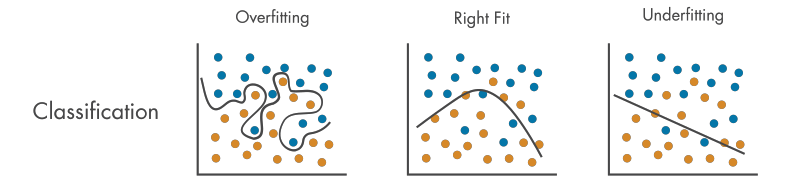
\includegraphics[width=0.9\textwidth]{img/overfiting-underfiting.png}
                  \caption{Comparación de sobreajuste e infrajuste. Imagen adaptada de \cite{mathworks-overfitting}}
                 \label{fig:overfiting}
        \end{figure}

Además, en un principio, se quería comparar sobre si clasificación binaria, era más eficiente que clasificación multiclase. Cuando se compararon estos valores, se utilizaba la medida ``accuracy'', que como ya se ha explicado no es recomendable su técnica en clasificación binaria. Aún así, se obtuvo resultados mejores en clasificación binaria que multiclase. Por ello, se decidió usar estos modelos.

En la gráfica \ref{fig:accuracy}, se observa el historial del mejor caso observado para la clasificación binaria.

        \begin{figure}[!ht]
                 \centering
                 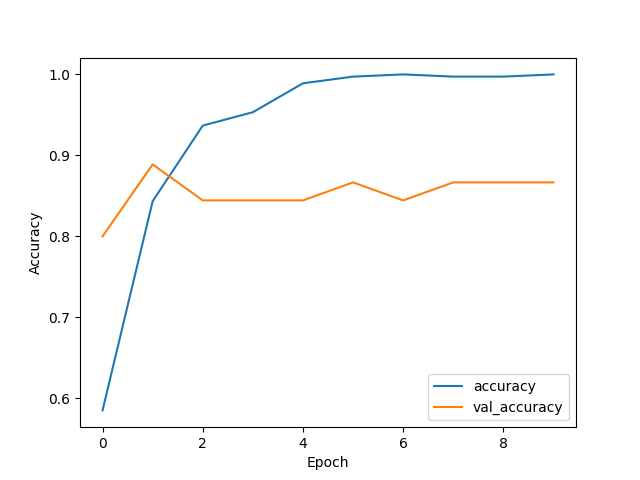
\includegraphics[width=0.5\textwidth]{img/modelo2-0.009int2_0.913043498992919920230525-172156.png}
                  \caption{Historial de la evolución de la ``accuracy''  de un modelo cuyo resultado de test era de 91\% }
                 \label{fig:accuracy}
        \end{figure}
Para obtener los nuevos modelos, con f1-score se volvió a ejecutar el código, pero, puesto que se observo que la clasificación binaria proporcionaba mejores resultados, se decidió comparar solo entre esta clasificación.

Al observar las matrices de confusión obtenidas, había 2 resultados mejores que los demás, y en varios casos, se obtuvo el resultado mencionado anteriormente, donde el modelo indicaba que todas las imágenes eran validas, pero en este caso, no se calculaba la ``accuracy''.

En la figura \ref{fig:comparacion de modelos}, se puede observar como y la matriz inferior, hace referencia al caso comentado, y las 2 matrices de confusión de la parte superior, hacen referencia a 2 modelos que clasifican de forma correcta casi todos los datos de test.

Para la matriz de la izquierda:
\begin{center}
    $Precision = \dfrac{11} {11 + 2} = 0.85 $

    $Recall = \dfrac{11} {11 + 0} = 1 $

    $F_1 = 2 \dfrac{0.85 * 1} {0.85 + 1} = 0.9189 $
\end{center}


Para la matriz de la derecha:
\begin{center}
    $Precision = \dfrac{10} {10 + 1} = 0.909 $

    $Recall = \dfrac{10} {10 + 1} = 0.909 $

    $F_1 = 2 \dfrac{0.909 * 0.909} {0.909 + 0.909} = 0.909 $    
\end{center}

Para la matriz de abajo:

\begin{center}
    $Precision = \dfrac{0} {0 + 0} = NaN $

    $Recall = \dfrac{0} {0 + 11} = 0 $

    $F_1 = 2 \dfrac{NaN * 0.909} {NaN + 0.909} = NaN $    
\end{center}
Entre las 2 opciones de la figura, aunque ambas han tenido la misma cantidad de aciertos, según la formula del f1-score, el modelo de la izquierda es mejor, puesto que acierta correctamente en todos los que predice como APTO, cosa que el modelo de la derecha no hace.

        \begin{figure}[!ht]
                 \centering
                 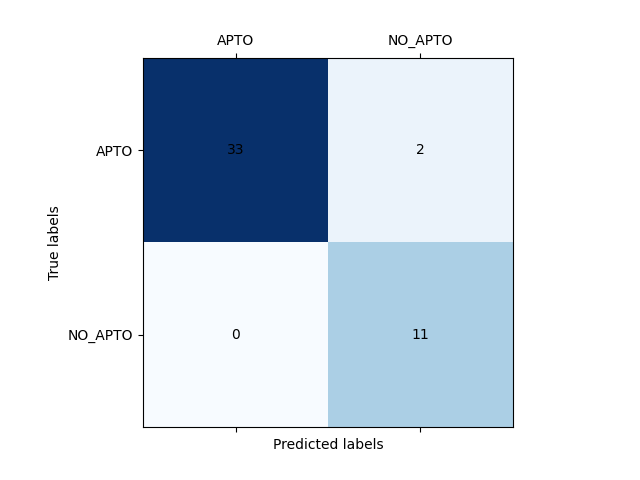
\includegraphics[width=0.45\textwidth]{img/modelo2-0.003int2_0.9166666720476415_20230603-003149.png}
                 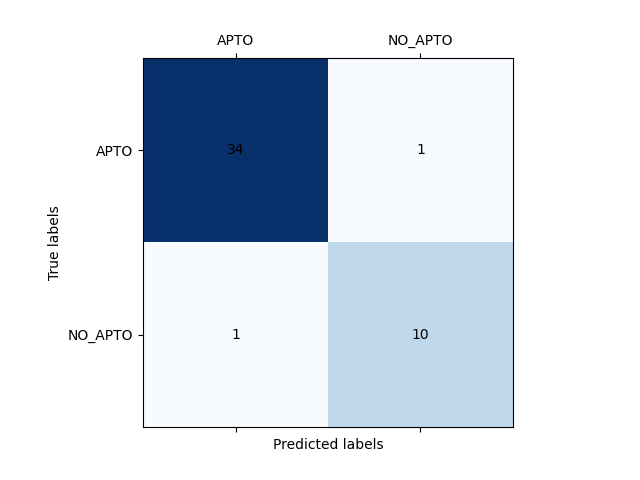
\includegraphics[width=0.45\textwidth]{img/modelo2-0.005int2_0.9090909361839294_20230603-010653.png}
                 \centering
                 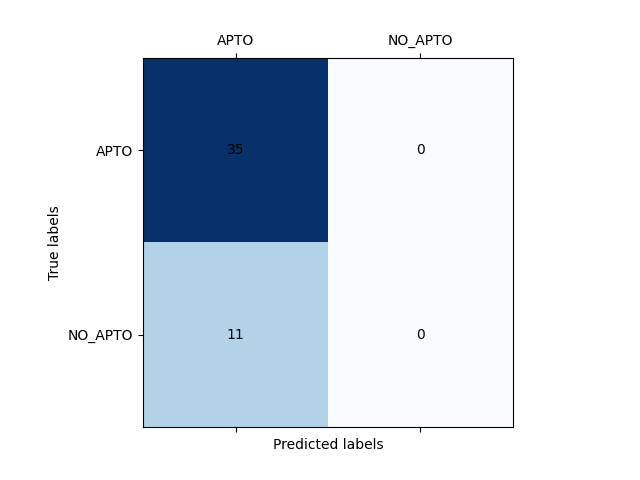
\includegraphics[width=0.45\textwidth]{img/modelo2-0.002int1_0_20230610-154306.png}
                  \caption{Comparación de los modelos destacables}
                 \label{fig:comparacion de modelos}
        \end{figure}

